% !TEX program = xelatex
\documentclass[12pt,a4paper]{article}
\usepackage[T1]{fontenc}
% --- XeLatex/LuaLatex ---
\usepackage[no-math]{fontspec}
\IfFontExistsTF{Fira Sans}{
	\setmainfont{Fira Sans}
}
\usepackage[indonesian]{babel}
\usepackage{booktabs}
%\renewcommand{\familydefault}{\sfdefault}
\usepackage{geometry}
\usepackage{tabularx}
\usepackage{graphicx}
\usepackage{float}
\usepackage{xcolor}
\usepackage{hyperref}
\usepackage{subcaption}
%\usepackage{subfigure}
\hypersetup{
	colorlinks=true,  % Colours links instead of boxes
	urlcolor=blue,    % Colour for external hyperlinks
	linkcolor=blue,   % Colour of internal links (sections, etc.)
	citecolor=red,    % Colour of citations
	bookmarks=true,   % Adds PDF bookmarks
	hypertexnames=true
}
\geometry{left=2cm, right=2cm, top=2cm}
\title{\textbf{Panduan Sinkronisasi Waktu dengan NTP Meinberg}}
\author{Observatorium Bosscha}
\hyphenation{me-la-ku-kan peng-amat-an deng-an di-re-ko-men-da-si-kan mem-pe-nga-ruh-i ren-tan peng-ambil-an}
\begin{document}
\maketitle
\noindent\rule{\linewidth}{0.4pt}
\begin{enumerate}
	\item Unduh file instalasi NTP Meinberg dari alamat berikut: \url{https://www.meinbergglobal.com/english/sw/ntp.htm}
	\begin{center}
		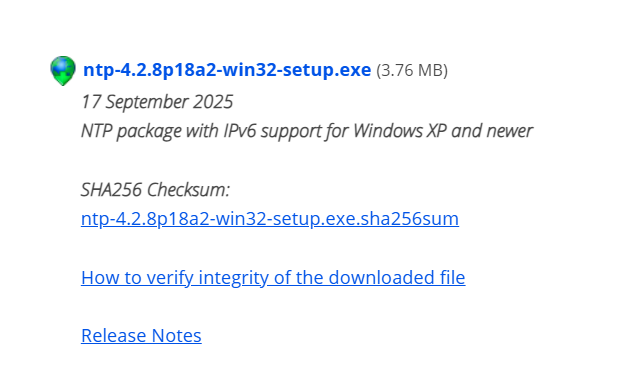
\includegraphics[width=0.5\linewidth]{ntp_download}
	\end{center}
	
	\item Klik ganda pada file, pilih \textbf{I Agree}.
	\begin{center}
		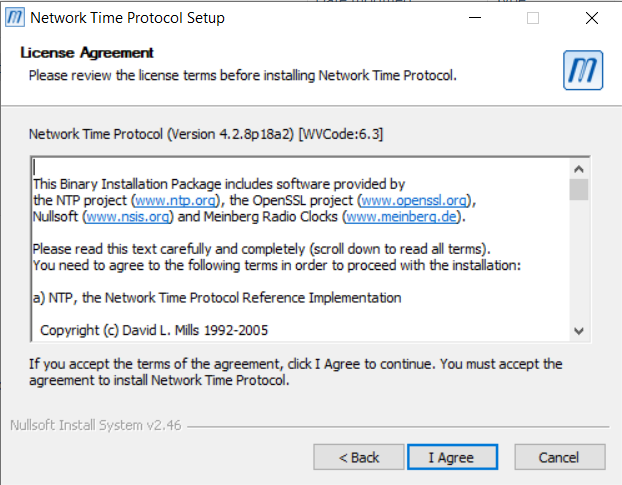
\includegraphics[width=0.5\linewidth]{ntp_agreement}
	\end{center}
	
	\item Tekan \textbf{Next}. Pada \textbf{Destination Folder} silakan tulis direktori tujuan instalasi, atau pilih default.
	\begin{center}
		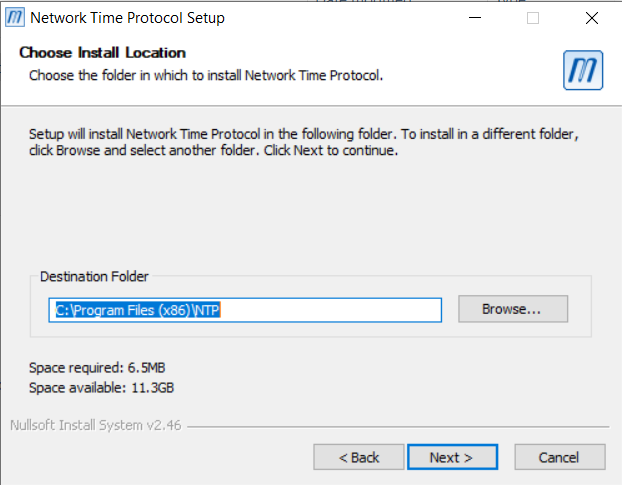
\includegraphics[width=0.5\linewidth]{ntp_install_dir}
	\end{center}
	
	\item Centang semua pilihan. Tekan \textbf{Next}.
	\begin{center}
		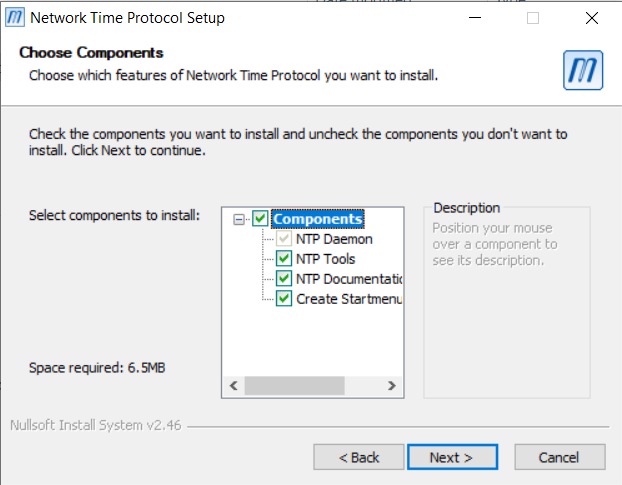
\includegraphics[width=0.5\linewidth]{ntp_components}
	\end{center}

	\item `Want to use predefined\ldots' pilih \textbf{Asia}.
	\begin{center}
		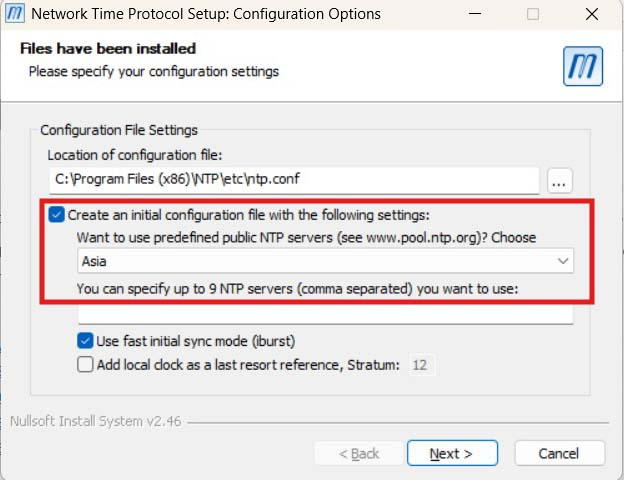
\includegraphics[width=0.5\linewidth]{ntp_config_options1}
	\end{center}
	
	\item Isi bagian di dalam kotak merah dengan NTP server pilihan anda (contoh:\\
	\texttt{ntp.bmkg.go.id}). 
	
	File konfigurasi ini bisa diedit terpisah nantinya pada direktori default:\\
	\textcolor{blue}{\path{Program Files (x86)/NTP/etc/ntp.conf}}\\
	(sesuaikan dengan direktori instalasi anda). Tekan \textbf{Next}.
	
	\begin{center}
		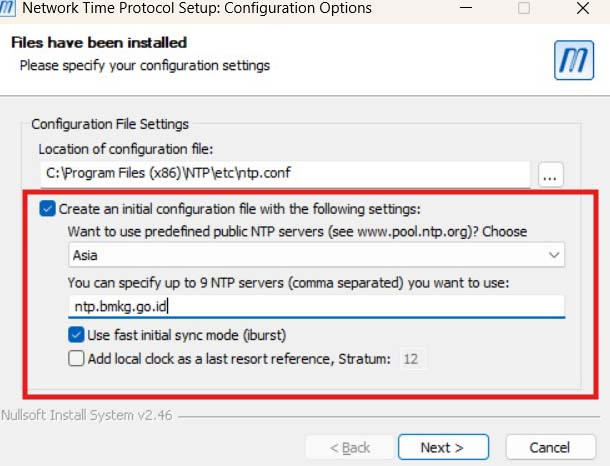
\includegraphics[width=0.5\linewidth]{ntp_config_options2}
	\end{center}
	
	\item Tekan \textbf{Next}. Jendela verifikasi config file akan muncul. Pilih \textbf{Yes} jika ingin melihat isi filenya, atau \textbf{No} untuk melihat dan mengeditnya di kesempatan yang berbeda.
	\begin{center}
		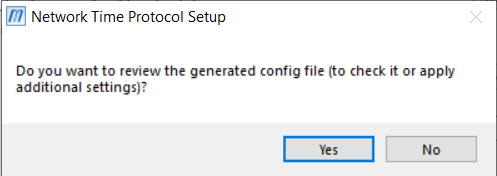
\includegraphics[width=0.5\linewidth]{ntp_review}
	\end{center}
	
	\item Jika memilih \textbf{Yes}, jendela berikut akan terbuka. NTP server yang dimasukkan pada poin 5 di atas akan tampil di file ini (lihat kotak merah). Copy dan Paste baris tersebut jika ingin menambahkan beberapa server lain. File config ini bisa diakses melalui direktori instalasi (lihat poin 5) dan mengeditnya dengan hak admin.
	\begin{center}
		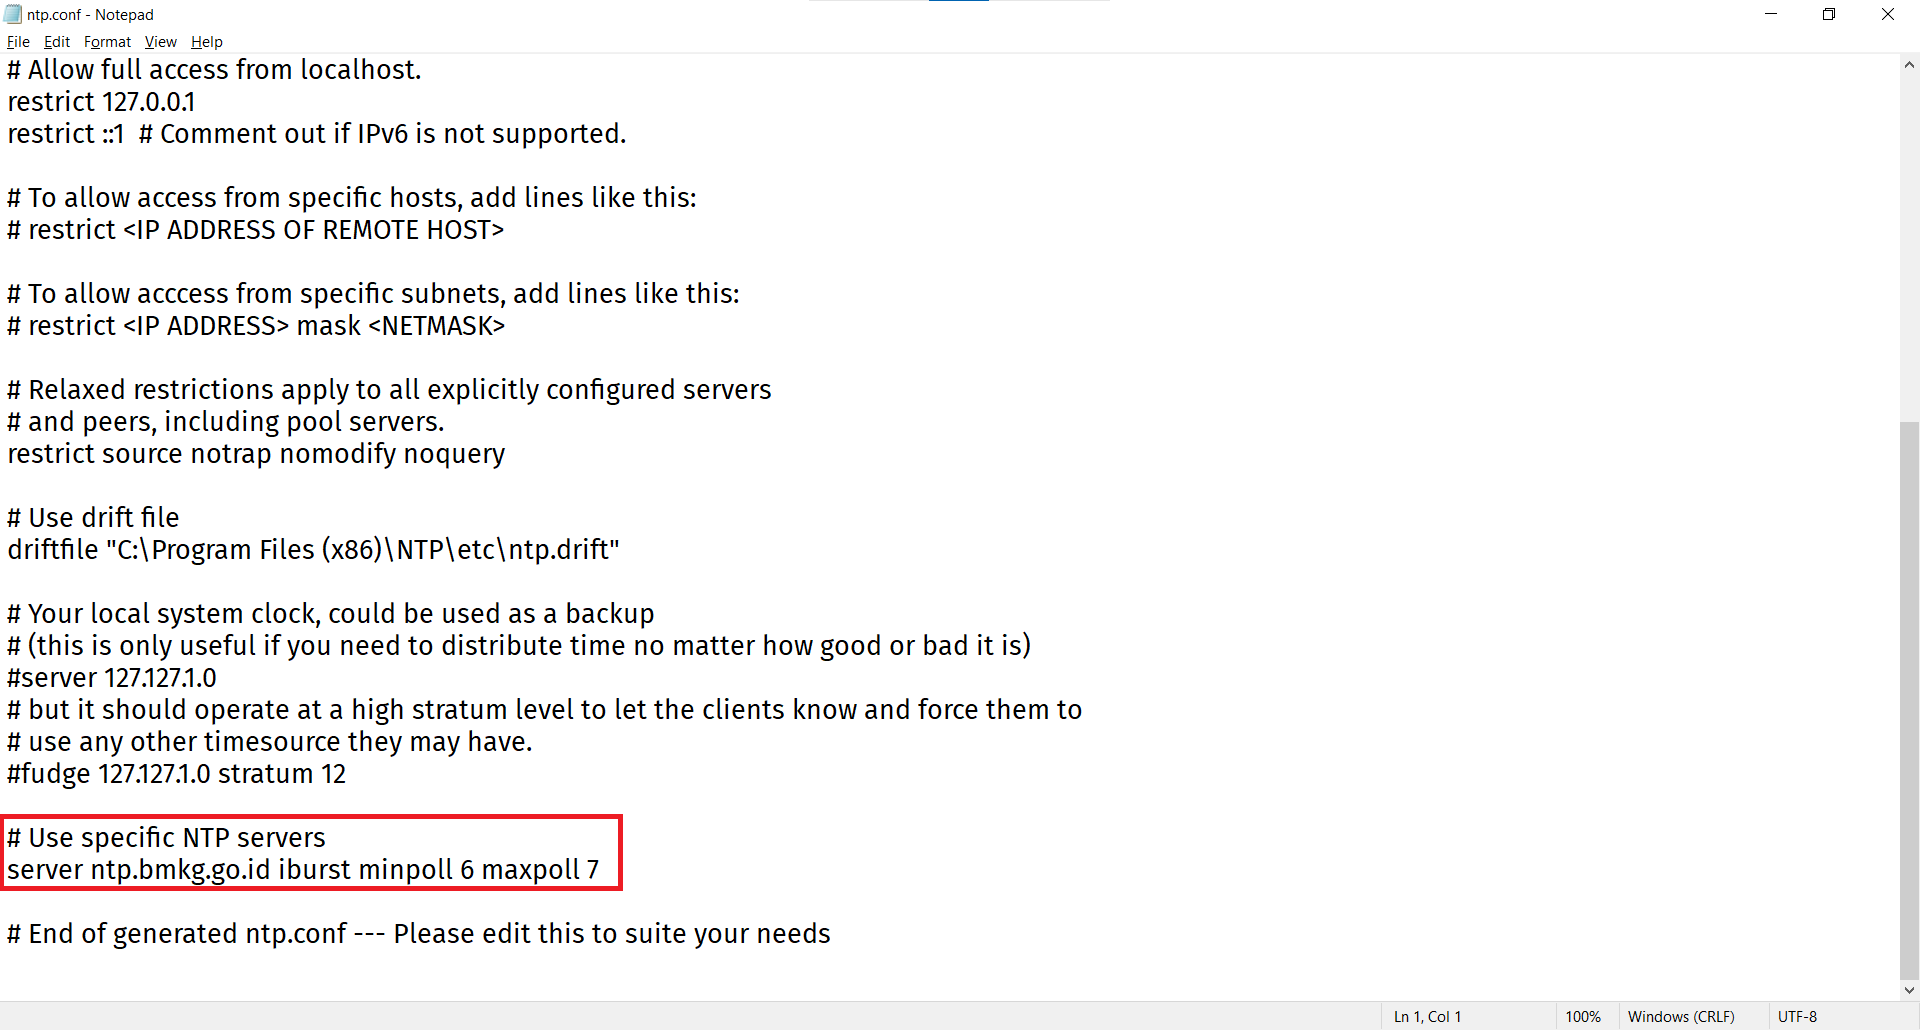
\includegraphics[width=0.7\linewidth]{ntp_conf_singleserver}
	\end{center}
	
	\item Sesuaikan seperti pada gambar. Tekan \textbf{Next}.
	\begin{center}
		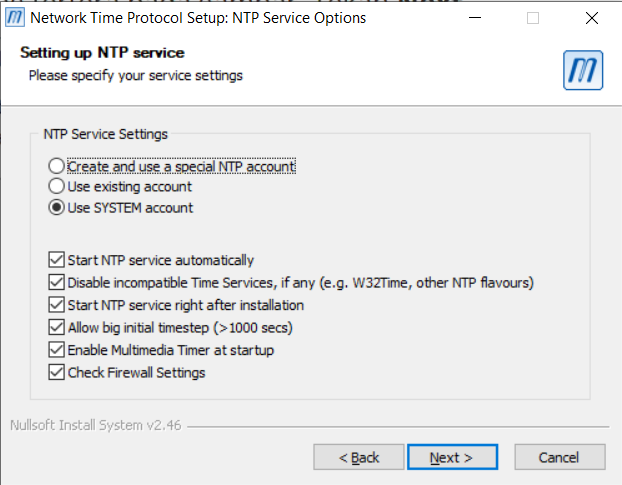
\includegraphics[width=0.5\linewidth]{ntp_service}
	\end{center}
	
	\item Tunggu instalasi selesai. Tekan \textbf{Finish}.
	\begin{center}
		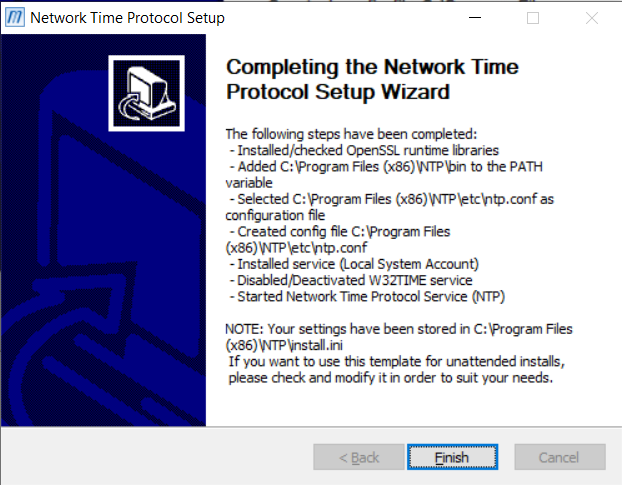
\includegraphics[width=0.5\linewidth]{ntp_finish}
	\end{center}
	
	
	\underline{Catatan}: Jika ingin menambahkan server NTP, edit file config pada mode \textbf{administrator} (lihat detil pada poin 7). Data server NTP, salah satunya, bisa dilihat pada \url{https://www.ntppool.org/en/} dan pilih zona yang diinginkan (misal Asia). Berikut adalah contoh penggunaan multi server pada file config.
	\begin{center}
		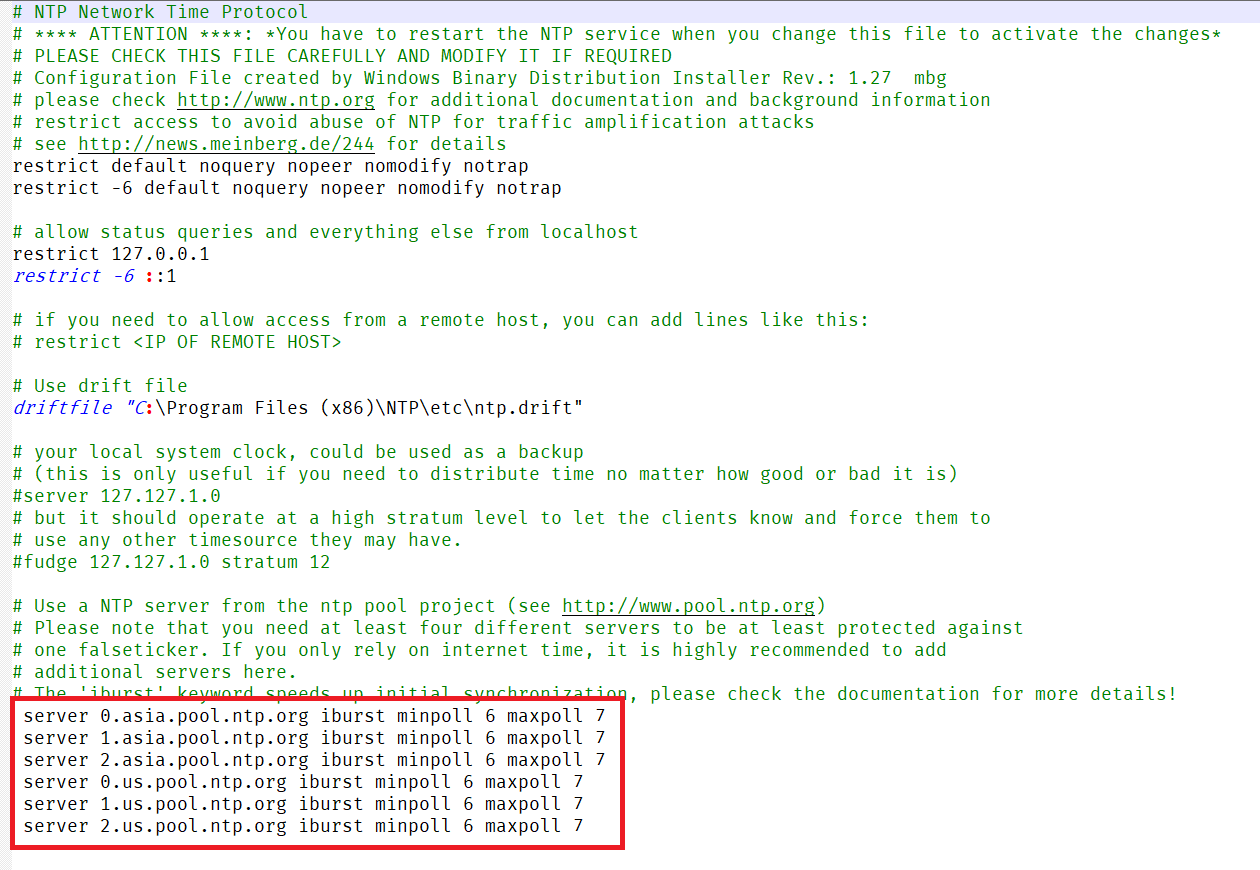
\includegraphics[width=0.7\linewidth]{ntp_conf}
	\end{center}
	
	\item Unduh dan instal NTP Client Monitor untuk memantau status sinkronisasi waktu. Aplikasi ini bisa diunduh dari \url{https://www.meinbergglobal.com/download/ntp/windows/time-server-monitor/ntp-time-server-monitor-104.exe}.
	
	\item Buka aplikasi NTP Client Monitor pada mode \textbf{Administrator}.
	 
	Masuk ke tab \textbf{NTP\allowbreak\_Status} untuk melihat status sinkronisasi waktu.
	\begin{center}
		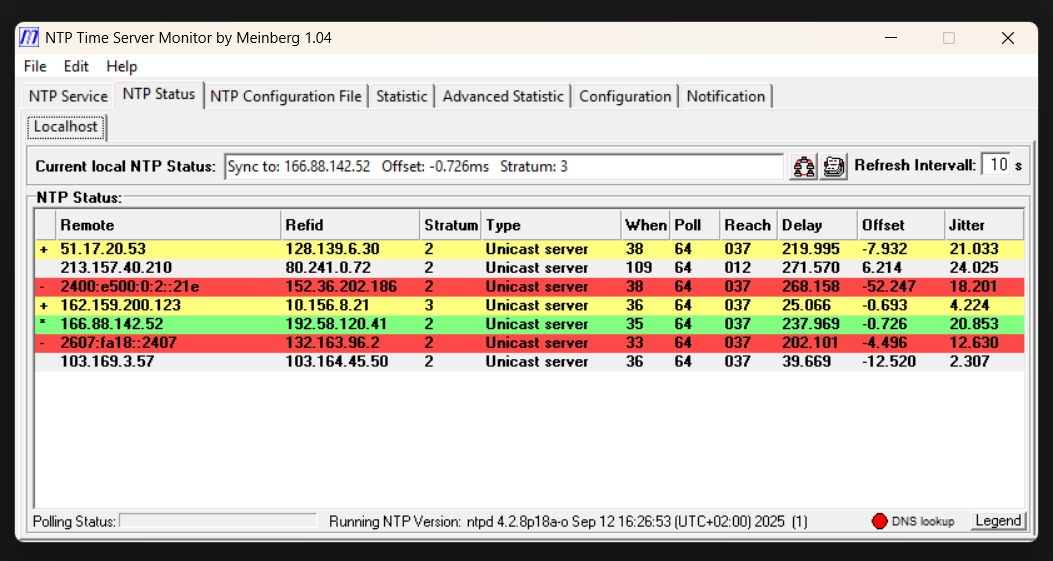
\includegraphics[width=0.5\linewidth]{ntp_status}
	\end{center}
	
	\item Tekan tombol \textbf{legend} untuk melihat arti dari setiap status sinkronisasi. Status `synchronized' dengan nilai \textit{offset} yang kecil (idealnya di bawah 1 ms) menunjukkan bahwa waktu komputer sudah tersinkronisasi dengan baik ke server NTP.
	\begin{center}
		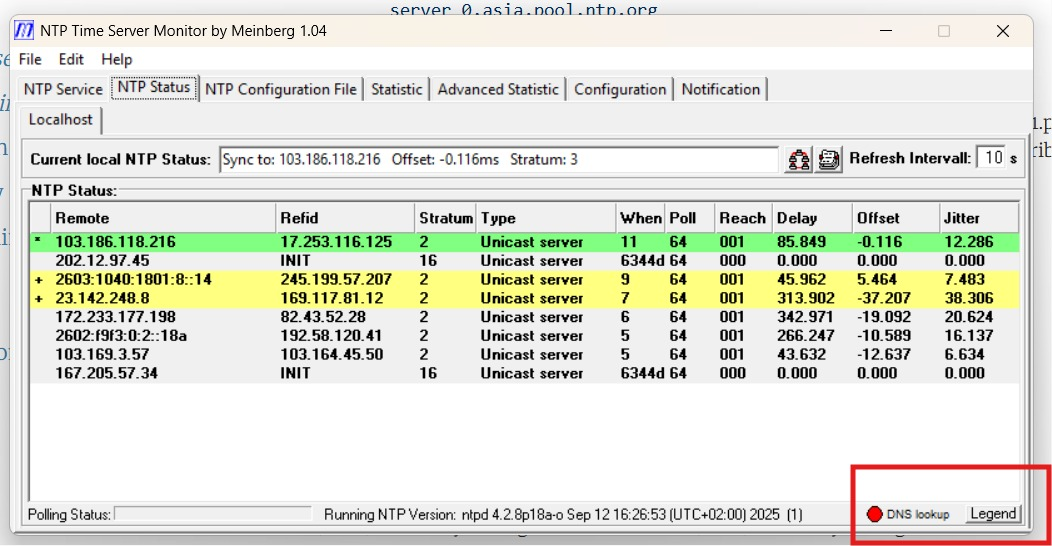
\includegraphics[width=0.5\linewidth]{ntp_legend}
	\end{center}
\end{enumerate}
\end{document}